\chapter{Streamlining the development of parallel algorithms using Noarr}
\label{chap:noarr}

% - many scientific algorithms are centered around a master data structure
%   - examples (matmul, transposition, physicell, ...)
% - the optimal run of these algorithms require an efficient memory traversal over the master data structure (both memory layout and traversal order) (both parallel and serial)
% - the domain experts usually can guess the optimal / close to optimal layout and traversal order
% - however, some optimizations require complex traversals that are very complex and error-prone to implement (tiling, levenstein, ...)
% - moreover, some traversting constants require tuning for different hardware (atlas)
% - other example is of a non expert who wants to speed up code by optimizing traversal - examples?
%   - there exist some dsls that can help with this
% - making this all by hand is very error-prone and time-consuming, unmantainable

% others do it too: cute, Kokos

% paper 1:
% - layout definition
% - allocation decoupling
% - layout agnostic
% - CUDA compatible
% - constants expressions
% - no overhead

% paper 2:
% - traversal definition / agnosticism
% - parallelism

Commonly, the core computation of scientific algorithms is centered around a master data structure. The examples include a matrix composed of cell features in an agent-based simulator~\cite{ghaffarizadeh2018physicell}, a grid of substrates in a diffusion solver~\cite{ghaffarizadeh2016biofvm}, a transition rates graph for Markov processes~\cite{koltai2020exact}, etc. In the vast majority of these algorithms, the location of the most performance-critical parts lies in a nested loop over these data structures.

Possibly due to the lack of hardware expertise, usually there is no special attention paid to the memory performance when such loops are written by the domain experts~\cite{clauss2000automatic}. As a result, the programs show poor data locality, spending most of the CPU cycles waiting for the memory pipeline to deliver the data.

A plethora of research works confirm that changing the way how data is laid in memory or modifying the nested loops can result in a significant performance improvement~\cite{gong2018empirical,stengel2015quantifying,serpa2019memory}. Such optimizations may include decreasing the number of cache misses by grouping the operation on the same data together, employing prefetching by streamlining the memory access pattern, or utilizing the vector instructions by aligning the data in memory. These optimizations are not exclusive to CPUs; they apply to GPUs similarly, further aiding in GPU-specific challenges, such as memory coalescing and utilizing memory hierarchies efficiently (as described in \cref{sec:gpu_arch}).

Arguably, given a nested loop to optimize, the expert in the performance optimization domain can pinpoint the biggest bottlenecks w.r.t. memory and propose close to optimal modifications with great probability. The most common modifications would include reordering the loops for the most possible serial access pattern and dividing the loops into tiles or strides to employ cache hierarchies~\cite{wolf1991data}. The problematic activity here, which takes the most programmers time, is putting these modifications into code. For example, let us have a nested loop of depth 3 with control variables \texttt{i, j, k} and bounds \texttt{I, J, K}. A simple tiling modification of the loop adds complexity in loop depth, variable count, and index computation:
\begin{minted}[fontsize=\footnotesize,breaklines,frame=leftline,linenos]{c++}
  for (i1 = 0; i1 < I / tile_I; i1++)
    for (j1 = 0; j1 < J / tile_J; j1++)
      for (k1 = 0; k1 < K / tile_K; k1++)
        for (i2 = 0; i2 < tile_I; i2++)
          for (j2 = 0; j2 < tile_J; i2++)
            for (k2 = 0; k2 < tile_K; k2++)
              // i=i1*tile_I+i2; j=j1*tile_J+j2; k=k1*tile_K+k2;
\end{minted}
Omitting corner cases, the code is already verbose and rather error-prone (a careful eye may spot a mistake, a usual copy-paste bug on Line~$5$).
Naturally, the complexity of the code grows with the complexity of the optimization.

Thankfully, many tools have been developed to alleviate this issue. Some provide automatic optimizations built within a compiler~\cite{trifunovic2010graphite,grosser2012polly}, some extend a compiler with pragma-like annotations to guide the optimization process~\cite{donadio2005language,yi2007poet,chen2008chill,namjoshi2016loopy} and others include ad-hoc solutions for a specific family of algorithms~\cite{9485033,AFANASYEV2021100707}. However, very little attention has been paid to aiding HPC programmers in writing the optimized code from scratch by providing them with a clean and maintainable way to express complex loop traversal and memory layout fit for their specific problem.

To alleviate and streamline the mundane programming tasks repeatedly encountered during our work on optimizing scientific algorithms, we focused our work on developing a C++ library \emph{Noarr}. The main benefit of the library is that it allows to expressively and extensively define memory layouts of regular $n$-dimensional arrays and provides loop transformation primitives for their optimal traversal. It empowers HPC experts to swiftly develop their optimizations as a clean, maintainable code open to autotuning and parallelism while staying within the borders of the C++ standard without adding any dependency on the final software product (which is an advantage for the deployment in a scientific community).

% Arguably, the biggest requirement for the optimal performance of these algorithms is such traversal over the master data structure that generates memory accesses in the most hardware-efficient way. This can either mean: the least number of cache misses, the best utilization of the memory hierarchy, loop unrolling, automatized vectorization. To have a brief perspective on the importance, a simple matrix transposition runs 50x faster when traverzing data in the right order.

% Critically, the expert int the performance optimization domain can usually guess the optimal or close to optimal traversal. In a big majority of cases, the proper cache utilization is just a question of iterating the loops in the right order and data tiling. The issue, which takes the most programmers time and is the most error-prone, is putting these traverals into code. A simple example of writing a tiling loop of 3D grid already results in an index hell.

% Furthermore, some optimizations require tuning of their parameters to be most efficient on a given hardware. For memory optimizations, such tunable parameters would be for example a size of a tile to fit given cache, or loop unrolling factor to sattisty the width of vector memory/compute instructions. Carrying out these tasks not in an automatized way is unmantainable and time-consuming. There are whole projects targeting automatic optimizations of specific algorithms, such as atlas for matrix multiplcation, FFTW for FFT, SPIRAL for signal processing. cuTLASS for CUDA matrix multiplication

% To alleviate and streamline these mundane programming tasks, which we encountered during our work on optimizing scientific algorithms multiple times, we focused our work here and developed a pure C++ library Noarr. Naturally, there are other libraries that aim to solve the same problem, the added value of noarr is:
% \begin{itemize}
%   \item a pure c++ approach without any need for DLS or precompilers. It empowers HPC experts to swiftly code their optimizations error-prone without adding any dependency on the final product. Which is usually paid huge attention to in a scientific community.
%   \item allows for simple tuning of the traversal constants for different hardware
%   \item CUDA compatible
%   \item support for parallelization of the traversal
%   \item %take sth from cgo paper
% \end{itemize}


\section{Memory Layouts}
\label{sec:layouts}

% - example of layout definition

% - example of traversal
% - how hard to define traversal by hand

% The main goal of noarr is to epressively and extensively define memory layouts and their traversals. There exists

% definition of layout
% definition of traversal
% they are isomorphic, but layout can be stronger than traversal eg thanks to vector instructions
% there are not many libraries that allow to easily define custom layout.
% there are some, which do just a specific use cases, such as Kokkos (which is a big library and is specialized just on a set of specific use cases) GridTools similarly
% but recently, in parallel with our research, bigger players started to realize the importance of memory layout. ndspan in c++ standard and cute in cuda. ndspan is a good start, but noarr is much more extensible. cute was developed for Atlas, but it is not as general as noarr.
% noarr defines layout by composing atom protostructs
% column major, row major example in double for loop
% perhaps example of transformation c->r
% we require traversal to do it effectively
% for traversals, there are way more other tools that do the same. some of them do it automatically, polly. many of them are, however, annotation based, requiring custom compiler to precompile the code. or compiler pragmas. They target a different audience. similar comparison is openMP vs tbb. https://link.springer.com/content/pdf/10.1007/978-3-642-03869-3_62.pdf While TBB appears to be less appropriate for parallelizing existing implementations, it fosters a good programming style and higher abstraction level for newly developed parallel programs.
% show noarr traverse - some split tile example ... perhaps physicell

Generally, the way how data is laid in memory, a \emph{memory layout}, can be portrayed as a projection of its index space to a linear memory space. If we limit ourselves to a general (non-ragged) $n$-dimensional array, we can define memory layout mathematically as follows:

\begin{defn}[Memory Layout]
 \label{def:layout}
 Suppose a regular $n$-dimensional array $A$ with dimension lengths $d_1, \dots, d_n$ and an index space $\mathcal{I} = \{0,\dots,d_1 - 1\}\times \dots \times \{0,\dots,d_n - 1\}$. We define a \emph{memory layout} $\mathbb{L}$ of $A$ as a bijection $\mathbb{L}: \mathcal{I} \to \{0,\dots, \prod_{i}d_i - 1\}$.
\end{defn}
Obviously, we are interested only in such bijections, that can be generated by straightforward mathematical formulas, such as in the following examples:

Perhaps the most common memory layouts are row-major and column-major of a matrix (Figures~\ref{fig:layout-row} and~\ref{fig:layout-col}). Their respective bijections can be generated by indexing functions $L_{\text{row}}(i,j) = i \cdot d_2 + j$ and $L_{\text{col}}(i,j) = j \cdot d_1 + i$ and these functions would be carried to source code with slight modifications.

As alluded to in the motivation, common layouts used to optimize memory accesses require a complex code. A tiled matrix layout (Figure~\ref{fig:layout-tile}), the layout paramount for some algorithms to optimally use cache hierarchies, already requires a verbose indexing function. Helping ourselves with adding two intra-tile dimensions, the indexing function would look as follows:
$$L_{\text{tiled}}(i,j,k,l) = (((i \cdot d_2 + j) \cdot d_3) + k) \cdot d_4 + l$$
Arguably, adding another tile dimension (to utilize multiple levels of cache or GPU memory hierarchy), swapping intra-tile layout to column-major form, or implementing layouts as space-filling curves (Figures~\ref{fig:layout-zcurve} and~\ref{fig:layout-hcurve}, especially useful when dealing with cache-oblivious algorithms~\cite{bader2006cache}) becomes less and less trivial. Moreover, considering the indexing functions are written ad-hoc, the layouts are tough subjects to change since a layout change requires a thoughtful and error-prone rewrite of all index function occurrences. On top of that, a complex indexing function is far from self-describing, making it hard, even close to impossible, to guess the layout intentions.

\begin{figure}[h]
  \centering
  \begin{subfigure}{.15\textwidth}
      \centering
      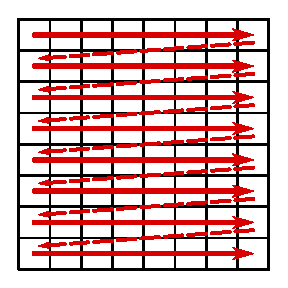
\includegraphics[width=.9\linewidth]{img/matrix-row-major}
      \caption{row-major}
      \label{fig:layout-row}
  \end{subfigure}
  \begin{subfigure}{.15\textwidth}
      \centering
      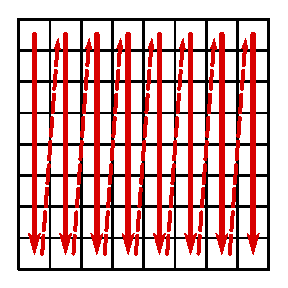
\includegraphics[width=.9\linewidth]{img/matrix-col-major}
      \caption{col-major}
      \label{fig:layout-col}
  \end{subfigure}
  \begin{subfigure}{.15\textwidth}
      \centering
      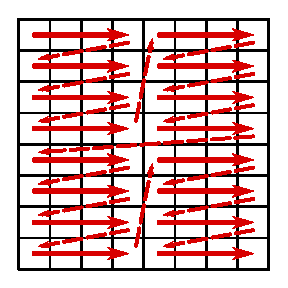
\includegraphics[width=.9\linewidth]{img/matrix-tiled}
      \caption{tiled}
      \label{fig:layout-tile}
  \end{subfigure}
  \begin{subfigure}{.15\textwidth}
      \centering
      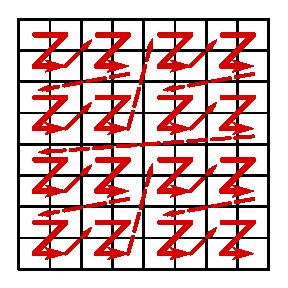
\includegraphics[width=.9\linewidth]{img/matrix-zcurve}
      \caption{z-curve}
      \label{fig:layout-zcurve}
  \end{subfigure}
  \begin{subfigure}{.15\textwidth}
      \centering
      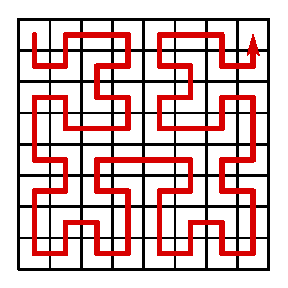
\includegraphics[width=.9\linewidth]{img/matrix-hcurve}
      \caption{Hilbert curve}
      \label{fig:layout-hcurve}
  \end{subfigure}
  \caption{Instances of various matrix layouts.}
  \label{fig:matrix-layout}
  \end{figure}

\subsection{Background}

The importance of these issues has been recognized by the HPC community, especially by the authors of HPC programming frameworks. Perhaps the oldest example is Kokkos~\cite{CARTEREDWARDS20143202}, a platform-agnostic programming model that defined a memory layout as a \emph{first-class object}. The layout is defined as a vector of dynamic dimension lengths; the dimensions are laid out in memory from left to right (the leftmost dimension being laid in the memory continuously with a stride of 1, also called Fortran-style), from right to left (perhaps the most used one, C-style) or generally by a custom vector of strides. Such a simple approach covers a wide range of HPC use cases and has been adopted by other frameworks, such as GridTools~\cite{AFANASYEV2021100707}. An example of defining a layout with $3$ dimensions of lengths $3$, $3$ and $4$ and their respective strides $1$, $5$ and $20$ in Kokkos is as follows:
\begin{minted}[fontsize=\footnotesize,breaklines,frame=leftline,linenos]{c++}
  // Some storage
  int* ptr = new int[80];
  // A layout object with pairs of size and stride
  Kokkos::LayoutStride layout(3, 1, 3, 5, 4, 20);
  // A view from the pointer and the layout
  Kokkos::View<int***> w(ptr, layout);
  int elem = w(0, 0, 0);
\end{minted}

Line~$6$ highlights another useful feature of the framework: The ability to decouple the layout from the underlying memory. The layout is a separate object from the memory pointer, which allows for easy reuse of the layout in different parts of the code. Connecting a layout to a memory is done explicitly by wrapping a layout and a memory pointer into a \texttt{View} object.

Recently, much bigger communities have started to invest time in designing an extensible way of defining layouts. C++ has standardized \emph{mdspan} in C++23. It takes a finer approach, allowing to define layout dimensions using a more complex extent structure. Such a structure enables defining some dimension lengths as static (known at compile time) and mixing them with some dynamic (known at runtime). With such information during compile-time, a compiler can employ optimizations such as constant folding, loop unrolling, or automatized vectorization. Similarly, as with a vector of strides in Kokkos, it defines a \texttt{LayoutPolicy}, responsible for converting dimensions to underlying 1D memory, and \texttt{mdspan} class as a \texttt{View} alternative:
\begin{minted}[fontsize=\footnotesize,breaklines,frame=leftline,linenos]{c++}
  // Some storage
  int* ptr = new int[80];
  // An extent structure, the first two dims are static
  std::extents<3, 3, std::dynamic_extent> ext(4);
  // mdspan object with a pointer, extents and Fortran-style layout policy
  std::mdspan<int, decltype(ext), std::layout_left> s(ptr, ext);
  int elem = s[0, 0, 0];
\end{minted}

Nvidia has recently introduced \emph{CuTe}, a collection of C++ CUDA template abstractions for defining and operating on hierarchically multidimensional layouts of threads and data~\cite{cute-online}. It follows similar principles as with the C++ standard: it defines \emph{shape}, \emph{stride}, and \emph{tensor} as alternatives to Extents, LayoutPolicy, and mdspan. The same example as above written using CuTe lists as follows:

\begin{minipage}{\textwidth - 18pt}
\begin{minted}[fontsize=\footnotesize,breaklines,frame=leftline,linenos]{c++}
  // Some storage
  int* ptr = new int[80];
  // A layout as a pair of shape and stride
  Layout l = make_layout(
    make_shape(Int<3>(), Int<3>(), 4),
    make_stride(Int<1>(), Int<3>(), Int<9>())
  );
  // A tensor object with a pointer and a layout
  Tensor t = make_tensor(ptr, l);
  int elem = t(0, 0, 0);
\end{minted}
\end{minipage}
\vspace{1pt}

Shapes and strides can be nested, creating a hierarchy of coordinates. Also, every layout (even a nested one) can be indexed with 1D coordinates, iterating the index space in a colexicografic order. This allows for a natural indexation of complicated layouts; e.g., a tiled matrix 4D layout can be indexed using standard 2D coordinates, hiding the complexity of the layout.
Apart from that, CuTe also takes a formal approach, creating a \emph{layout algebra}. It defines a set of operations over layouts, such as concatenation, composition, tiling, and others. These operations are used to build more complex layouts from simpler ones.

% CuTe - much more formal approach - defines a layout algebra
% more complex layout able to "hide dimensions"
% more complex stride, which does not have to

% If you're familiar with the C++23 feature mdspan, this is an important difference between mdspan layout mappings and CuTe Layouts. In CuTe, Layout is a first class citizen, is natively hierarchical to naturally represent functions beyond row-major and column-major, and can similarly be indexed with a hierarchy of coordinates. (mdspan layout mappings can represent hierarchical functions as well, but this requires defining a custom layout.) Input coordinates for an mdspan must have the same shape as the mdspan; a multidimensional mdspan does not accept 1-D coordinates.

% CuTe provides an "algebra of Layouts" to support combining layouts in different ways. This algebra includes operations such as

% Layout functional composition,
% a notion of Layout "product" to reproduce one layout according to another, and
% a notion of Layout "divide" to split one layout according to another.
% Common utilities for building complicated layouts from simpler ones depend on the Layout product. Common utilities for partitioning layouts (of data, for example) across other layouts (of threads, for example) depend on the Layout divide. All of these utilities rely on the functional composition of Layouts.

% In this section, we'll build up the tools of the Layout algebra and explain some of these core operations in detail.

% The developers familiar with this issue by encapsulating the memory layout into a complete object representing a data structure. Kokkos, platform-agnostic programming model, provides a simple syntax to define a list of static or dynamic dimensions of a multi-dimensional regular array and allows user to specify if the dimensions should be layed in memory from left to right (C-style), from right to left (Fortran-style) or in a custom stride.
% GridTools provides a similar functionality, but it is more focused on the stencil computations and allows to select back-ends (GPU, multicore-CPU, \dots) according to which the most suitable layout will be selected. However, the memory layout is a very general concept and it is impossible to cover all the use-cases.

% The mentioned works are mainly focused on a generalized optimization of a specific set of algorithms. They implement ways to efficiently parallelize problems, distribute and aggregate data. Still, they discovered that memory layout is integral part of the optimization process. Hence, they integrated some freedom of layout selection as a part of their libraries.

% Standalone layouting stuff:
% In parallel with our research, other works have been done in this area. C++ standard introduces mdspan, which will provide basic layouting functionality in standard library as soon as C++23 with more coming C++26. NVIDIA also realised the importance of extensive layouts and introduced CuTe library with a simmilar layouting algebra.
% %https://arxiv.org/html/2312.11918v1/#S3

\subsection{Noarr Layouts}

Our contribution \emph{Noarr} aims to enhance the expressiveness, extendibility, and maintainability of the code. The main points which distinguish Noarr from other libraries are:

\begin{itemize}
  \item \emph{Named dimensions} --- the dimensions are not defined just by an order of shape or stride vectors, but they are named. This allows to query a dimension regardless of its global index.
  \item \emph{Proto-structures} --- a set of building blocks is provided to allow to easily define complex layouts by their various composition.
\end{itemize}

Let us give an example of a row-major matrix memory layout using Noarr. Considering \mintinline{c++}{'i'} as a row dimension and \mintinline{c++}{'j'} as a column dimension, the layout can be defined as follows:

\begin{minted}[fontsize=\footnotesize,breaklines,frame=leftline,linenos]{c++}
  // Some storage
  int* ptr = new int[80];
  // A row-major matrix layout
  auto row_l = scalar<int>() ^ vector<'j', 'i'>(lit<3>, 4);
  // A bag object with a pointer and a layout
  bag b = make_bag(row_l, ptr);
  int elem = b.at<'i', 'j'>(0, 0);
\end{minted}

Although Noarr predates mdspan and CuTe, it shares many similarities: the separation of layout and underlying memory (using \texttt{bag} on Line~$6$) and the ability to define static and dynamic-sized dimensions (using \texttt{lit} on Line~$4$). Perhaps the biggest difference is the absence of a stride vector. In Noarr, the strides are computed automatically according to the order of the named dimensions. The matrix layout above can be changed to column-major by a simple named dimensions swap:
\begin{minted}[]{c++}
auto col_l = scalar<int>() ^ vector<'i', 'j'>(4, lit<3>);
\end{minted}
The order in which the dimensions are defined signals the way how they are laid in memory, which is in the left-to-right fashion. The meaning of the dimension names is important here, as it determines the \emph{logical order}. The order in the definition then defines the \emph{physical order}. For example, let us have a cube layout, denoting its height, width and depth as \mintinline{c++}{'i'}, \mintinline{c++}{'j'} and \mintinline{c++}{'k'} respectively. A C-style cube layout could be defined using \mintinline{c++}{vector<'k', 'j', 'i'>()} proto-structure. A custom layout (neither Fortran- nor C-style) can be simply written as \mintinline{c++}{vector<'j', 'k', 'i'>()}. Using this logical--physical distinction, all of the vastly used stride vectors can be simulated by permuting the dimensions order.

The other aspect of Noarr is the way how the layout is defined --- as a composition of building blocks, the protostructures. We already mentioned \texttt{row\_l}, which is a composition of \mintinline{c++}{scalar<int>} and \mintinline{c++}{vector<'j', 'i'>}, which, when composed, represents a vector (\mintinline{c++}{'i'}) of vectors (\mintinline{c++}{'j'}) of integer scalars (\mintinline{c++}{int}) --- an integer matrix. The left-to-right reading of the layout definition allows for easy extension of the existing layout. Let us enumerate examples of more complex layouts in the following listing.

\begin{minted}[fontsize=\footnotesize,breaklines,frame=leftline,linenos]{c++}
  // A layout for a batch of row-major matrices
  // and offset to the 1st row of the 2nd matrix
  auto batched_l = row_l ^ vector<'b'>(10);
  size_t o1 = batched_l | offset<'i', 'j', 'b'>(1, 0, 2);
  // Two tiled matrix layouts (both row-major and col-major,
  // where 'k' and 'l' denote tile rows and columns)
  auto tiled_rr_l = row_l ^ vector<'l', 'k'>(5, 10);
  auto tiled_rc_l = row_l ^ vector<'k', 'l'>(10, 5);
  // A sublayout composed of the 3rd row tiles
  auto tiled_3rd_l = tiled_rc_l ^ fix<'k'>(3);
  // A tiled matrix layout indexable using 2 coordinates
  auto tiled_2d_l = tiled_rr_l ^ merge_blocks<'i', 'k', 'I'>() ^ merge_blocks<'j', 'l', 'J'>();
\end{minted}

The protostructures allow for expressing complex layouts in a readable and verifiable way. Furthermore, their extensibility in composition and separation from the underlying memory also allows for plug-in layouts, which can be easily \emph{reused} in different parts of the code:

Let us have a complex layout of a multi-layered 3D grid gradient, which occurs on various code places and provides layouts for multiple memory pointers. In that case, a layout can be declared once with sufficient scope and reused in places where needed:

\begin{minted}[fontsize=\footnotesize,breaklines,frame=leftline,linenos]{c++}
  // A globally accessible layout
  auto gradient_layout = scalar<float>()
    ^ vector<'s', 'x', 'y', 'z', 'g'>(
      substrates, grid_dims[0], grid_dims[1], grid_dims[2], lit<3>
    );

  void func1_cpu(float* grad_ptr) {
    bag b = make_bag(gradient_layout, grad_ptr);
    // use the layout on CPU memory
  }

  void func2_gpu(float* global_mem_ptr) {
    bag glb_b = make_bag(gradient_layout, global_mem_ptr);
    bag shm_b = make_bag(gradient_layout, shared_mem_ptr);
    // use the layout on GPU global and shared memory
  }
\end{minted}

The other benefit of having a layout as a reusable first-class object is the ability to have a localized change when deciding to modify the layout code during the implementation. Extending our previous example, if we decide to reorder the gradient dimension \mintinline{c++}{'g'} to be the innermost one, we only change the definition of the object on Line~$2$ --- all the data structures using the layout will be transparently updated without any further code changes.


% Noarr puts the biggest emphasis on expressiveness, performance, and extensibility of memory layouts. It is a standalone C++ header-only library based on template metaprogramming and is based on these principles:
% \begin{itemize}
%   \item \emph{named dimensions} The dimensions are not defined just by an order of some numbers, but they are named. This allows to query info of a dimension regardles its global index.
%   \item \emph{trivial layouts} A set of trivial layout transformers is provided to allow to easily define complex layouts by composition of simple transformations.
% \end{itemize}

% Noarr borrows trivial tranformations from a well-known set of loop transformation, but extends it with some more. These are dimension reordering,
% strip mining, fusion, fission, but also a z-curve

% Let us give an example of row-major matrix memory layout using noarr. Considering \mintinline{c++}{'i'} as a row dimension and \mintinline{c++}{'j'} as a column dimension, the layout can be defined as follows:
% \begin{minted}[breaklines]{c++}
% auto row_major = scalar<float>() ^ sized_vector<'j'>(n) ^ sized_vector<'i'>(m);
% \end{minted}
% The layout reads from left to right, signaling the innermost dimension first.
% It is apparent, that \mintinline{c++}{row_major} object represents only a layout, and to access the data, a memory pointer has to be provided:
% \begin{minted}[breaklines]{c++}
% float* data = new float[n * m];
% float element = row_major | get_at<'i', 'j'>(data, 0, 0);
% \end{minted}
% To define a column-major layout, preserving the semantics of the dimension name, the layout can be defined as follows:
% \begin{minted}[breaklines]{c++}
% auto col_major = scalar<float>() ^ sized_vector<'i'>(m) ^ sized_vector<'j'>(n);
% \end{minted}
% The layout can be modified even more by introducing multiple dimensions. For example, to define a tiled layout, we add two more dimensions for the tiles:
% \begin{minted}[breaklines]{c++}
% auto tiled = scalar<float>() ^ sized_vector<'l'>(tile_n) ^ sized_vector<'k'>(tile_m) ^ sized_vector<'j'>(n / tile_n) ^ sized_vector<'i'>(m / tile_m);
% \end{minted}
% Here shows the power of named dimensions. Physically (in memory), \mintinline{c++}{'l'} and \mintinline{c++}{'k'} dimensions are innermost, representing column and row of a tile respetively. Dimensions \mintinline{c++}{'j'} and \mintinline{c++}{'i'} are outermost, representing column and row of a matrix, whose elements are whole tiles. With such semantics, tiles are both among themselves and within in row-major format. Unsurprisingly, the inter-tile layout can be changed to column-major by a simple rewrite:
% \begin{minted}[breaklines]{c++}
%   auto tiled = scalar<float>() ^ sized_vector<'k'>(tile_m) ^ sized_vector<'l'>(tile_n) ^ sized_vector<'j'>(n / tile_n) ^ sized_vector<'i'>(m / tile_m);
% \end{minted}


\section{Traversing Layouts}
\label{sec:traversals}

Having specified how a data structure is laid in memory, the other possible point of optimization lies in the order how the data structure is iterated, its \emph{traversal}. In general, a traversal is usually written as a sequence of nested loops, which in turn generates a sequence of data structure accesses. Using such interpretation, we define the traversal of a layout as follows:

\begin{defn}[Layout Traversal]
 \label{def:traversal}
 Suppose a sequence of $n$ nested loops with the loop boundaries $d_1, \dots, d_n$ and a memory layout of a data structure with an index space $\mathcal{I}$. We define a \emph{layout traversal} $\mathbb{T}$ as a bijection $\mathbb{T}: \{0, \dots, \prod_{i}d_i - 1\} \to \mathcal{I}$.
\end{defn}

In conjunction with the memory layout from Definition~\ref{def:layout}, a natural observation arises: $\mathbb{L}$ and $\mathbb{T}$ are composable, and their composition $\mathbb{L} \circ \mathbb{T}$ is a function \emph{from integers to integers} --- it generates the memory access pattern. As a corollary, the same sequence of accesses can be generated by either changing the layout ($\mathbb{L}$) or its traversal ($\mathbb{T}$). Therefore, as with a layout, modifying a traversal can improve data locality, both in time and space. Although modifying traversal can be constrained by data dependencies, loop transformation is still a well-researched topic and complements the memory layout optimization~\cite{clauss2000automatic}.

Writing complex traversals complements the issues discussed above when detailing the layouts. So, such tool can share the same benefits: expressivity, maintainability, and reusability. Moreover, since traversing over some master data structures is the common place where parallelism is introduced in the code, the abstraction of loop transformation can further extend to parallel processing.

\subsection{Background}

Quantitatively, \emph{loop transformation} is perhaps a more researched topic than layout transformation. Neither library mentioned above provides ways to transform a traversal, but many other tools do. Contemporary compilers employ sophisticated loop optimizers based on the polyhedral model, such as Graphite in GCC~\cite{trifunovic2010graphite} or Polly in LLVM~\cite{grosser2012polly}. However, these optimizers are limited by the lack of information specified by the user in the code.

For more user-guided approaches, there are annotation-based tools, such as Poet~\cite{yi2007poet}, Chill~\cite{chen2008chill} or Loopy~\cite{namjoshi2016loopy}. These tools allow to specify the traversal transformations by adding special comments or pragmas to the code. The transformations are then applied by a precompiler, which generates the optimized code. Perhaps the best representative of annotation-based frameworks is done by Kruse et al.~\cite{kruse2018user}. The authors have presented pragma-based user-directed loop transformations for the Clang compiler, which has been partly adopted by the OpenMP standard. The transformations include loop tiling:
\begin{minted}[fontsize=\footnotesize,breaklines,frame=leftline,linenos]{c++}
  // original code
  #pragma clang loop(i,j) tile sizes(4,8)
  for (int i = 0; i < n; i+=1)
    for (int j = 0; j < m; j+=1)
  // transformed code
  for (int i1 = 0; i1 < n; i1+=4)
    for (int j1 = 0; j1 < m; j1+=8)
      for (int i2 = i1; i2 < n && i2 < i1+4; i2+=1)
        for (int j2 = j2; j2 < m && j2 < j1+8; j2+=1)
\end{minted}
or loop reordering:
\begin{minted}[fontsize=\footnotesize,breaklines,frame=leftline,linenos]{c++}
  // original code
  #pragma clang loop(i,j) interchange permutation(j,i)
  for (int i = 0; i < n; i+=1)
    for (int j = 0; j < m; j+=1)
  // transformed code
  for (int j = 0; j < m; j+=1)
    for (int i = 0; i < n; i+=1)
\end{minted}
but also loop fusion, fission, reversal, and others~\cite{mckinley1996improving}.

These tools are straightforward to use, and their ability to combine them to form complex loop transformations makes them very expressive. A minor downside is that they are typically closed to extensions, and for most of them, a precompiler with an extra preprocessing step or a custom compiler extension is needed.

On the other hand, the target problems for annotation-based loop transformation tools are somehow limited. Naturally, the best use of them is made when there is already a baseline implementation, and the optimization is achieved just by adding a few lines on the top of the loop with the hottest performance spots. However, when developing an optimized solution from scratch and when the scale of the program passes a certain complexity threshold, optimizing just by annotations may become cumbersome.

A good evidence of this fact is case studies that compared the effort of programming a parallel algorithm using OpenMP, also a pragma-based library, with pure C++ libraries, such as TBB. The studies generally confirm that ease of expressing parallelism in OpenMP is traded for a lower abstraction level and flexibility. Language-based approaches, such as TBB, can utilize object-oriented design for more control, fostering of good programming style and higher abstraction level for \emph{newly} developed parallel programs~\cite{kegel2009using,ajkunic2012comparison,refsnes2011comparison}.

\subsection{Noarr Traversers}

The similarities in memory layout and its traversal led us to the development of our following contribution, \emph{Noarr Traversers}. The tool is based on the idea that every single loop, in some sequence of nested loops, can be interpreted as one (named) dimension in an index space domain. Assuming perfectly nested loops, such traversal can be interpreted as a Noarr layout and be subjected to the same transformations as a memory layout. To sum up, the key points of Noarr Traversers are as follows:
\begin{itemize}
  \item \emph{Named dimensions} --- a traverser comprises named dimensions, each representing a loop in a sequence of nested loops.
  \item \emph{Proto-structures} --- exactly as with layouts, a traverser is subject to an extension using the same set of proto-structures.
  \item \emph{Index space extraction} --- the traverser extracts dimensions from the passed-in layouts and yields an index space corresponding to the cartesian product of the extracted dimensions.
\end{itemize}

Let us highlight the main idea of Noarr Traverser on an example of matrix multiplication, where a plain C++ implementation would look like this:

\begin{minted}[fontsize=\footnotesize,breaklines,frame=leftline,linenos]{c++}
  for (int i = 0; i < m; i++)
    for (int j = 0; j < n; j++)
      for (int k = 0; k < p; k++)
        C[i][j] += A[i][k] * B[k][j];
\end{minted}
The nested loops follow the order of $3$ present dimensions: $i$, $j$, and $k$ denoting rows of $C$ and $A$, columns of $C$ and $B$, and rows of $A$ and columns of $B$, respectively. Smartly selecting the named dimensions of the layouts, the traversal can be rewritten using Noarr as follows:

\begin{minted}[fontsize=\footnotesize,breaklines,frame=leftline,linenos]{c++}
  auto A = make_bag(ptr_a, scalar<int> ^ vector<'k', 'i'>(K, I));
  auto B = make_bag(ptr_b, scalar<int> ^ vector<'j', 'k'>(J, K));
  auto C = make_bag(ptr_c, scalar<int> ^ vector<'j', 'i'>(J, I));

  traverser(A, B, C) | [=](auto state) {
    C[state] += A[state] * B[state];
  };
\end{minted}
The traverser accepts the layouts (or bags) it shall iterate over. It extracts $3$ unique dimensions \mintinline{c++}{'i'}, \mintinline{c++}{'j'} and \mintinline{c++}{'k'} and iterates over the index space composed of these dimensions as if they were written as a sequence of nested loops (which is equivalent to the cartesian product of these dimensions). The lambda function on Line~$6$ is then executed for each point in the index space, passing the tuple of indices as the \texttt{state} argument to the lambda.

Thanks to the dimension naming, traversers and layout objects are also \emph{isomorphic}. Consequently, changing the traversal order is done the same way as modifying the layout --- by applying the proto-structures to the traverser. E.g., to reorder the loops to a more cache-friendly \mintinline{c++}{'i'}, \mintinline{c++}{'k'}, \mintinline{c++}{'j'} order, the traversal can be rewritten as follows:
\begin{minted}[fontsize=\footnotesize,breaklines,frame=leftline,linenos]{c++}
  traverser(A, B, C) ^ reorder<'i', 'k', 'j'>() | [=](auto state) {
    C[state] += A[state] * B[state];
  };
\end{minted}
Furthermore, a side product of the isomorphism is that a proto-structure can be applied either to the layout or to the traverser, granting the same effect.

Let us conclude the benefits of tracking loops by names with a more complex example:
Some transformations change the nesting level of the underlying loops, e.g., during a strip-mine transformation, where a loop is split into two nested loops by a blocking factor~\cite{mckinley1996improving}. Following the Noarr paradigm of named dimensions, a strip-mine is well defined by a proto-structure \mintinline[fontsize=\footnotesize]{c++}{into_blocks}, which accepts the first dimension as the input, which should be present in the layout, and two output dimension, which will be newly added to the composed layout. Since all loops are tracked by their names, the user has full control over the output of a transformation and can safely chain multiple transformations together. Tiled matrix multiplication can be expressed as follows:

\begin{minipage}{\textwidth - 18pt}
\begin{minted}[fontsize=\footnotesize,breaklines,frame=leftline,linenos]{c++}
  // breaking dimension 'i' into two new dimensions 'I' and 'x'
  auto tiles = into_blocks<'i', 'I', 'x'>(noarr::lit<16>)
             ^ into_blocks<'j', 'J', 'y'>(noarr::lit<16>)
             ^ into_blocks<'k', 'K', 'z'>(noarr::lit<16>)
             // using the new dimensions
             ^ reorder<'I', 'J', 'K', 'x', 'y', 'z'>();

  traverser(A, B, C) ^ tiles | [=](auto state) {
    C[state] += A[state] * B[state];
  };
\end{minted}
\end{minipage}

\subsection{Reusability}

Similarly as with layouts, a specific traversal order can be defined as an object, such as \texttt{tiles} on Line~$2$ in the previous code sample, and provide the same benefits: locality of change and reusal.

But this feature further extends to a perhaps more powerful concept, which we call \emph{layout agnosticism} and \emph{traversal agnosticism}. As a case of the separation of concerns, a memory layout and traversal can be extracted from a function to the level of function arguments. These arguments may then serve as interfaces for the concrete traversal or layout objects:

\begin{minted}[fontsize=\footnotesize,breaklines,frame=leftline,linenos]{c++}
  template <class A_t, class B_t, class C_t, class Order_t>
  void matmul(A_t& A, B_t& B, C_t& C, Order_t my_order)
  {
      traverser(A, B, C) ^ my_order | [=](auto state) {
          C[state] += A[state] * B[state];
      };
  }
\end{minted}
The function \mintinline{c++}{matmul} becomes agnostic to the layout or traversal specified, and, regardless of the passed-in objects, it will run the same operations, just in a different order.

The modular template-based design of Noarr allows us to mimic the autotuning systems, which search the vast space of transformation, trying to find the most performant one for a specific computational function. In our approach, we may be able to express precisely that with the traversal-agnostic and layout-agnostic functions.

\subsection{Parallelism}

Since Noarr is general enough to allow the division of traversals into independent sub-traversals, the user can also guide the parallelism of a program. Proto-structures such as \mintinline{c++}{fix}, \mintinline{c++}{slice} or \mintinline{c++}{step} provide expressive ways to split a work over a data structure into custom sections. The user can then assign each section to a separate thread, which will iterate over the section independently.

But if the user wants to offload this task to a well-known field-tested parallel library, Noarr is also open to this extension. Our modular design allows us to plug in various \emph{parallel executors}. So far, we experimented with OpenMP, TBB, and CUDA, extending the library with parallel-for, parallel-reduce, and others. The parallel \texttt{for-each} using Noarr and OpenMP can be written as follows:

\begin{minted}[fontsize=\footnotesize,breaklines,frame=leftline,linenos]{c++}
  // parallelising over dimension x
  #pragma omp parallel for
  for (auto t_inner : a_traverser ^ hoist<'x'>()) {
    t_inner | [=](auto state) { /* ... */ }; // some independent work
  }
\end{minted}

The code sample further strengthens the benefit of named dimensions: The user can directly specify the dimension to parallelize over. This is even more visible when targeting parallel accelerators (such as GPUs) in which a programmer can select multiple dimensions to utilize thread hierarchies (as described in \cref{sec:gpu_arch}):

\begin{minted}[fontsize=\footnotesize,breaklines,frame=leftline,linenos]{c++}
  auto A = make_bag(ptr_a, scalar<int>() ^ vector<'x', 'y'>(32, 1000));
  // spawns a cuda block for each element of the 'y' dimension
  // with as many threads as the size of 'x' dimension
  auto ct = noarr::cuda_threads<'y', 'x'>(traverser(A));
  a_kernel<<<ct.grid_dim(), ct.block_dim()>>>(ct.inner(), A);

  __global__ void a_kernel(auto traverser, auto A) {
    // A is accessed according to the block index
    // and the thread index of the currently executing thread
    auto var = A[traverser.state()];
  }
\end{minted}

\section{Summary}

With the arsenal of proto-structures, Noarr provides options to specify many complex layouts and traversals. The object-oriented design of the library allows writing complex memory optimizations in an extensible, reusable, and even layout-agnostic way, with very little space for errors. Further, the pure C++ implementation enables the usage of Noarr in C++-based frameworks, such as CUDA. The library has already been incorporated into our ongoing work of implementing a high-performance version of BioFVM~\cite{ghaffarizadeh2016biofvm}, a diffusion solver for 3D biological simulations, aiding in various loop transformations, vectorization, dividing the data into subdomains for parallelization, and other optimizations, all realized in a clean and self-documenting way\footnote{The code is available from the GitHub repository https://github.com/asmelko/paraBioFVM}.

We believe that our solution will add a new expressive tool to a high-performance programming toolset, simplifying the research focusing on tuning of prewritten computational kernels and building complex optimized parallel algorithms from scratch.

% \section{Auto-tuning and parallelism}

% A common benefit of the aforementioned annotation-based loop transformers is the ability to automatically search the transformation space and find the most optimal traversal. This process of \emph{autotuning} is especially useful when the code is supposed to run on different hardware. As an example, the different cache sizes or vector registers widths can be easily adapted to by the autotuning process~\cite{frigo1998fftw,puschel2004spiral,whaley1998automatically}.

% The modular template-based design of Noarr allows us to mimic the autotuning systems. It is achieved by defining a layout or a traversal as an argument of a performance-critical function. That way, a function is agnostic of the layout or traversal specified and, regardless the passed-in layout, it will result in the same operations, just in a different order. Such layout-agnostic (or traveral-agnostic) functions can be called repeatedly with different combinations of layout and traversal transformations. Listing~\ref{lst:agn} shows an example of a transformation-agnostic function written using Noarr, used to generate a performance heatmap of the benchmarked transformations (Figure~\ref{fig:heatmap_all}).

% \begin{listing}
%   \begin{minted}[fontsize=\footnotesize,breaklines]{c++}
%   template <class A_t, class B_t, class C_t, class Order_t>
%   void matmul(A_t& A, B_t& B, C_t& C, Order_t my_order)
%   {
%       traverser(A, B, C) ^ my_order | [=](auto state) {
%           C[state] += A[state] * B[state];
%       };
%   }
%   \end{minted}
%   \caption{Layout- and traversal- agnostic matrix multiplication.}
%   \label{lst:agn}
% \end{listing}

% \begin{figure}
%   \centering
%   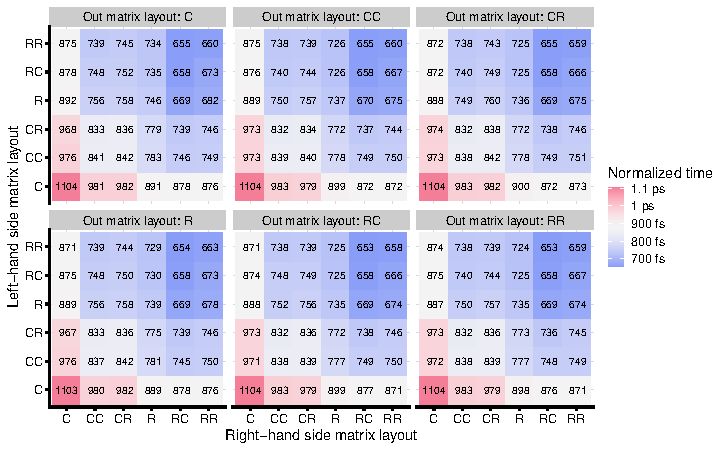
\includegraphics[width=0.8\textwidth]{img/heatmap_all}
%   \caption{Heatmap of the execution time of a matrix multiplication algorithm with different layout transformations. The optimal transformation is highlighted in blue.}
%   \label{fig:heatmap_all}
% \end{figure}

% Lastly, Noarr is compatible with parallelism. Noarr proto-structures are general enough to allow division of layouts and traversals into sublayouts and subtraversals for user-guided parallelism. Moreover, Noarr supports parallelization wrappers around TBB, OpenMP and CUDA, managing the division of the specified dimensions and assigning their traversal to parallel workers automatically.


% In the future, we plan to combine the proposed innovations
% with autotuning methods. The traversal-agnostic functions
% should provide an exciting starting point for the automated
% exploration of various traversal orderings. Furthermore, we
% are experimenting with using the layout-agnostic paradigm
% with the ultimate goal of designing a self-adaptive system
% that could change the layout of the data structures or even
% the order of loops at runtime.



% \subsection{layout agnostic code}

% Benefits of some annotation-based tools is the ability to automatically search transformation space and find the most optimal traversal. Such \emph{autotuning} is especially useful when the code is supposed to run on different hardware. The different cache sizes or vector registers widths can be easily adapted to by the autotuning process.

% As first-class objects, noarr layouts and traversals allow for \emph{layout-agnostic} and \emph{traversal-agnostic} code. A code, which contains the performance critical part, such as nested for loop of a scientific algorithm, can be encapsulated in a function, with traversal and layout extracted into function parameters:
% \begin{listing}
%   \begin{minted}[fontsize=\footnotesize,linenos,breaklines]{c++}
%   template <class A_t, class B_t, class C_t, class Order_t>
%   void matmul(A_t& A, B_t& B, C_t& C, Order_t my_order)
%   {
%       traverser(A, B, C).order(my_order).for_each([&](auto Aidxs, auto Bidxs, auto Cidxs)
%       {
%           C.at(Cidxs) += A.at(Aidxs) * B.at(Bidxs);
%       });
%   }
%   \end{minted}
%   \caption{Traversal-agnostic matrix multiplication}
%   \label{lst:agn}
% \end{listing}

% The function can be called repeatedly with a different combination of layout and traversal transformations. Benchmarking the differently parametrized functions then shows the optimal transformations on a running hardware and highlights the most effective optimizations on a general hardware.

% % add figure heatmap_all


% The modular template-based design of this extension al-
% lows us to mimic the autotuning systems, which search the
% vast space of transformation, trying to find the most per-
% formant one for a specific computational function. In our
% approach, we may be able to express precisely that with
% so-called traversal-agnostic functions — the body of such
% functions does not change, although the traversal order does
% (see Listing 7).

% Our approach may promote less time spent in code compiling as we do not require to modify the source code when applying the different transformations. However, this is farfrom the scope of this paper.

% benefits of some of annotation based tools is the ability to autotune some layout parameters
% noarr layout agnostic abstraction allows just the same
% example of layout agnostic
% code can run irrespective the traversal used (assuming the traversal is correct)(isomorphic)
% find sth from cgo paper


% \section{parallelism}

% parallelism is a different kind of beast, it can alter the traversal
% considering algorithms with master data structures, the parallelism is usually a question of in which nested loop are we aiming to parallelize
% there can be caveats ofcourse, such as data dependencies, but they are usually easy to spot
% there can be caveats, such as different hierarchies of parallelsim (either be it simd on CPUs or more prevalent GPU) - so there is a need to divide in multiple levels
% noarr traversals are general enough to do this in a custom way
% nevetherless, we experimented with wrappers around tbb to provide proof of concept
% wrapper around cuda kernel launch which divides over 2 dims
% structure for cuda shared mem?
% examples





% na zaciatok 2.2. viac popisat uzitocnost - uzitocnost para
% ako 2.3.4 pridat aj paralelizmus